\documentclass[a4paper, 12pt]{article}
\usepackage{epsfig}
%\usepackage{caption}
\usepackage{subcaption}
\usepackage{amssymb}
\usepackage{graphicx}
%\usepackage[export]{adjustbox}
\usepackage{pdfpages}
\usepackage{wrapfig}
\usepackage[margin=1.0in]{geometry}
\usepackage{amsmath}

\begin{document}
\title{Study of the shock front and solitary profile of electron acoustic wave in a weakly relativistic plasma in critical limit}
\author{DD-Leader\\nlpl931\\Sudip}
\date{\today}
\maketitle
%\tableofcontents
\newpage
\section{Abstract}
\label{Abstract}
% This is a comment. COmments start with '%'. These are single line only.
Using the quantum hydrodynamic model, the Korteweg–de Vries Burgers (KdVB) type solitary structures of electron acoustic waves(EAWs) have been analytically studied, in a homogeneous, isotropic, non-magnetised plasma consisting of two electron temperatures with a weak relativistic degeneracy. The dispersion relation for such waves has been derived, and the effect of various plasma parameters(Quantum diffraction H,density related parameter $\delta$,relativity parameter $\beta$,viscosity $\eta$) has been thoroughly investigated. The KdVB equation is derived in an extreme limit using the popular reductive perturbation technique, and the effect of quantum diffraction,Mach Number,unperturbed electron velocity on the resulting travelling shock wave solution have been studied by simulation models and hence an observation on the formation and propagation of shock waves is made.
\newpage %starts whatever after it, on the next page.
\tableofcontents % This starts in a new page due to the above command.
\newpage
\section{Introduction} % Creates the introduction tag.
A plasma is a quasineutral gas of charged and neutral particles which exhiibits collective behaviour. While individual single particle like behaviour is dominant in low density plasmas, the fluid like behaviour is also visible in high density plasma, such as those present in the upper atmosphere. Hence, the motion of fluid elements is taken into account for such cases, although much different from the usual fluid dynamics, due to the involvement of electric and/or magnetic fields. In the fluid approximation, the plasma is composed of two or more
interpenetrating fluids, one for each species, such as ions, electrons, or neutrals. Even multiple species of electrons or ions are possible depending upon the energy (temperature equivalent). Due to the presence of charged particles, a plasma couples to electric and magnetic fields and because of the collective fluid like behaviour plasma supports a wide variety of wave phenomena.
\newline % Starts writing on a new line. Like a paragraph...
The electromagnetic fields in a plasma are assumed to have two parts, one static/ equilibrium part and one oscillating/perturbation part. Waves in plasmas can be classified as electromagnetic or electrostatic according to whether or not there is an oscillating magnetic field. Acoustic waves in plasmas are primarily electrostatic. This means the magnetic filed is constant, or zero. In this paper, the propagation of electron acoustic waves are explored. For such a wave, the ions are considered to be stationary and infinitely heavy while electrons oscillate.  Moreover these waves can be formed only when two different electron pooulations exist, typically referred to as hot and cold electrons. These oscillations are high frequency, although it is less than plasma frequency. The restoring force is due to the pressure of the hot electrons, while the cold electron component provide the inertia. The phase velocity of these electron acoustic waves is much higher than the thermal velocities of both cold electrons and ions, yet much smaller compared to the thermal velocity of the hot electrons.\cite{akter}
\newline
Plasmas which are not in thermal equilibrium exhibits two-temperature electrons,such plasmas are found in laboratory experiments\cite{armst,diti,kadom} i.e., fusion devices, sputtering magnetron plasma, and laser-plasma interaction experiments and space environments\cite{and,bame}.e., solar wind, earth’s bow shock, near interplanetary shocks, planetary and neutron star magnetosphere etc.\cite{manta}The importance of EAW related structures in different astrological situation has been reported by various spacecraft missions\cite{roth}(e.g., FAST at the auroral regions, GEOTAIL and POLAR missions in the magnetosphere).In classical plasma where de-Broglie wavelength associated with the plasma particles is very much less than the size of the system,they can be treated as pointlike objects but in quantum plasma the de-Broglie wavelength of the charged carriers become comparable to the spatial scale of the plasma system and then quantum effects become crucial and hence QHD model is introduced,which is actually the extensions of usual classical fluid model in plasmas, where a quantum correction term, the so-called “Bohm potential,” appears in the equation of motion for the charged particles.\cite{haas,manta}.Also in high density plasma the thermal pressure of the high velocity electrons become negligible compared to the Fermi degeneracy pressure,which arises due to the Puali’s exclusion principle.Under such extreme conditions,electrons can attain the speed of light in vacuum.So,in such cases both degeneracy and relativity has to be considered.\cite{sc}
\newline
Perturbation techniques which has been first developed in 19th century for astronomical applications is now considered to be a standard tool for the analysis of non-linearity of dynamical systems.In this technique,the system variables are expanded in terms of a small parameter $\epsilon$ and the unperturbed value of the variable.The reductive perturbation technique(RPT developed in \cite{gard}) ,which is mainly used in case of small amplitude non-linear waves was  first extensively used in determining the solitary wave characteristics of ion acoustic wave in \cite{watanabe} .Here,with some rescaling stretched variables are introduced in terms of a small parameter $\epsilon$ and the phase velocity $V_0$ of the solitary acoustic wave.Along with the stretching,the expansion of flow variables and taking terms upto small order($2^{nd}$,$3^{rd}$) perturbations KdV,KdVB or with different stretching mKdV,mKdVB equations are obtained.
\newline
The purpose of the present paper is to look into the effect of different parameters(Quantum diffraction H,density related parameter on the dispersion relation $\delta,\beta$) on the discontinuous dispersion relation in the long wavelength region and to graphically investigate and comment on the formation of small shock waves(ripples) and the time evolution of a stationary shock wavefront ,considering a different stretching of coordinates used in \cite{sc}.Also the effect of the above mentioned parameters on the motion of the mkdv solution(positive and negative) is shown graphically.The results may be used in understanding behaviour of EAW in dense quantum plasma,treated in a critical region.
\section{Mathematical Treatment}
\label{maths}
\subsection{Basic Equations}
\label{basic}
The following basic equations have been used.
Assuming that the region of treatment is closed, the continuity equations for hot and cold electrons are as follows:
\newline
\begin{equation}
    \frac{\partial n_h}{\partial t} + \frac{\partial (n_h u_h)}{\partial x} = 0
\end{equation}
\begin{equation}
    \frac{\partial n_c}{\partial t} + \frac{\partial (n_c u_c)}{\partial x} = 0 
\end{equation}

The hot electrons have enough energy such that they are more mobile and hence are not bound by the typical fluid equations. Hence...
\newline
\begin{equation}
     0 = \frac{1}{m_e} [e \frac{\partial \phi}{\partial x} - \frac{1}{n_h}\frac{\partial P_h}{\partial x} + \frac{\hbar^2}{2m_e}\frac{\partial}{\partial x}[\frac{1}{\sqrt{n_h}}\frac{\partial^2 \sqrt{n_h}}{\partial x^2}]] 
\end{equation}
\newline
The cold electrons are moving slowly enough (lower energy) that they are under the effect of the main oscilations. Hence,
\newline
\begin{equation}
    (\frac{\partial}{\partial t} + u_c \frac{\partial}{\partial x})u_c = \frac{1}{m_e}[e\frac{\partial \phi}{\partial x} + \frac{\hbar^2}{2m_e}\frac{\partial}{\partial x}
    [\frac{1}{\sqrt{n_c}}\frac{\partial^2 \sqrt{n_c}}{\partial x^2}] + \eta_c \frac{\partial^2 u_c}{\partial x^2}]
\end{equation}
\newline
And finally since we are considering acoustic waves, the poisson equation is still valid. So, the poisson equation for cold, hot electrons and ions is as follows:
\newline
\begin{equation}
    \frac{\partial^2 \phi}{\partial x^2} = 4\pi e (n_c + n_h - Z_i n_i) 
\end{equation}
\newline
The equation of state is basically a side product of weak relativistic degeneracy. Thus the pressure depends non linearly on the density of hot electrons.
It is as follows:
\newline
\begin{equation}
  P_j = \frac{1}{20}{{(\frac{3}{\pi}})}^{\frac{2}{3}} (\frac{h^2}{m_e}) {n_j}^{\frac{5}{3}}
\end{equation}
\subsection{Normalization}
\label{normalize}
The quantities in the equations need to be normalized, in order to make the Mathematical Treatment easier. This means using certain fixed quantities to make the equations dimensionless.
The following Normalization procedure is used:\newline
\newline
\begin{math}
    t \rightarrow t\omega_{pc},\quad
    x \rightarrow x\frac{\omega_{pc}}{V_{Feh}},\quad
    u_j \rightarrow \frac{u_j}{V_{Feh}},\quad
    n_j \rightarrow \frac{n_j}{n_{j0}},\quad
    \phi \rightarrow \frac{e\phi}{2k_B T_{Feh}},\quad
    \eta_c \rightarrow \eta_c \frac{\omega_{pc}}{{V_{Feh}}^2 m_e}
\end{math}
\newline
\newline
Where $\omega_{pc}$ denotes the plasma frequency of cold electrons, and $V_{Feh}$ denotes the Fermi velocity of the hot electrons. So, $V_{Feh} = \sqrt{\frac{2k_B T_{Feh}}{m_e}}$ and thus,
$\omega_{pc} = \sqrt{\frac{4\pi e^2 n_{ec0}}{m_e}}$. A quantum diffraction ends up being present, which is denoted by $H = \frac{\hbar \omega_{pc}}{2k_b T_{Feh}}$. Using the above, the normalized equations end up as:
\begin{equation}
    \frac{\partial n_h}{\partial t} + \frac{\partial n_h u_h}{\partial x} = 0 \label{cont-h}
\end{equation}
\begin{equation}
    \frac{\partial n_c}{\partial t} + \frac{\partial n_c u_c}{\partial x} = 0 \label{cont-c}
\end{equation}
\begin{equation}
    0 = \frac{\partial \phi}{\partial x} - \frac{\beta}{{n_h}^\frac{1}{3}}\frac{\partial n_h}{\partial x} + \frac{H^2}{2}\frac{\partial}{\partial x}
    [\frac{1}{\sqrt{n_h}}\frac{\partial^2 \sqrt{n_h}}{\partial x^2}] \label{mom-h}
\end{equation}
\begin{equation}
    (\frac{\partial}{\partial t} + u_c \frac{\partial}{\partial x})u_c = \frac{\partial \phi}{\partial x} + \frac{H^2}{2}\frac{\partial}{\partial x}
    [\frac{1}{\sqrt{n_c}}\frac{\partial^2 \sqrt{n_c}}{\partial x^2}] + \eta_c \frac{\partial^2 u_c}{\partial x^2} \label{mom-c}
\end{equation}
\begin{equation}
    \frac{\partial^2 \phi}{\partial x^2} = n_c + \frac{n_h}{\delta} - \frac{\delta_1 n_i}{\delta} \label{poisson}
\end{equation} 
\newline
Where $\delta = \frac{n_{c0}}{n_{h0}}$ and $\delta_1 = \frac{Z_i n_{i0}}{n_{h0}}$ are the ratios of the equilibrium concentrations of cold electrons, hot electrons and ions respectively.\\
And $\beta = \frac{1}{12}({\frac{3n_{h0}}{\pi}})^\frac{2}{3}(\frac{h^2}{2k_B m_e T_{Feh}})$

\subsection{Dispersion Relation}
The equilibrium values of all electron/ion concentrations and $\phi$ are taken to be uniform, so that the study of the wave like behaviour is done through perturbations about these equilibrium values. However this is not applicable for ions since they are heavier than electrons and hence assumed to be inertial.
Consequently, the following perturbation scheme is used.
\begin{eqnarray}
    n_j &=& 1 + \epsilon {n_j}^{(1)} + \epsilon^2 {n_j}^{(2)} + \dots \\
    u_j &=& u_0 + \epsilon {u_j}^{(1)} + \epsilon^2 {u_j}^{(2)} + \dots \\
    \phi &=& \phi_0 + \epsilon \phi^{(1)} + \epsilon^2 \phi^{(2)} + \dots
\end{eqnarray}
Hence, to find the linear dispersion relation, the relations among the first order terms are obtained \dots\\
The continuity equation gives (for hot and cold electrons respectively):
\begin{equation}
    (\omega - u_o k) {n_j}^{(1)} = k {u_j}^{(1)}    
\end{equation}
Now considering the momentum equation for the hot electrons, only the first order terms in the Taylor expansion of $\sqrt{n_h}$ and ${n_h}^{\frac{-1}{3}}$ are retained, giving the following:
\begin{equation}
    \phi^{(1)} = (\beta + \frac{H^2 k^2}{4}){n_h}^{(1)}    
\end{equation}
Carrying out the same thing for the momentum equation of the cold electrons,
\begin{equation}
    -(\omega - u_0 k){u_c}^{(1)} = k \phi^{(1)} - \frac{H^2 k^3}{4}{n_c}^{(1)} + ik^2 \eta_c {u_c}^{(1)}    
\end{equation}
where, $i = \sqrt{-1}$. This indicates that the dispersion relation is complex, i.e, k is a complex quantity and in general damping is to be expected.
Finally, the Poisson equation for the hot and cold electrons reveals,
\begin{equation}
    -k^2 \phi^{(1)} = {n_c}^{(1)} + \frac{{n_h}^{(1)}}{\delta}
\end{equation}

Solving these linear relations, the following dispersion relation is obtained:
\begin{equation}
\label{dispersion-final}
    \frac{\delta(\beta k^2 + \frac{H^2 k^4}{4})}{1 + \delta (\beta k^2 + \frac{H^2 k^4}{4})} = {(w - u_0 k)}^2 - \frac{H^2 k^4}{4} + i \eta_c k^2 (w - u_0 k)
\end{equation}
Since the factor $i=\sqrt{-1}$ is present in the above equation, it implies the presence of a complex dispersion relation between $\omega$ and k. As such, the wave vector $k$ is complex and can be written as $k_r + i\kappa$. Hence the dispersion relation has a real and an imaginary part. The imaginary part implies damping. Figures \ref{disp-var1} show the variation of the real part of the dispersion relation with respect to the plasma parameters.
\begin{figure}[t]
    \begin{subfigure}{0.5\textwidth}
    \centering
    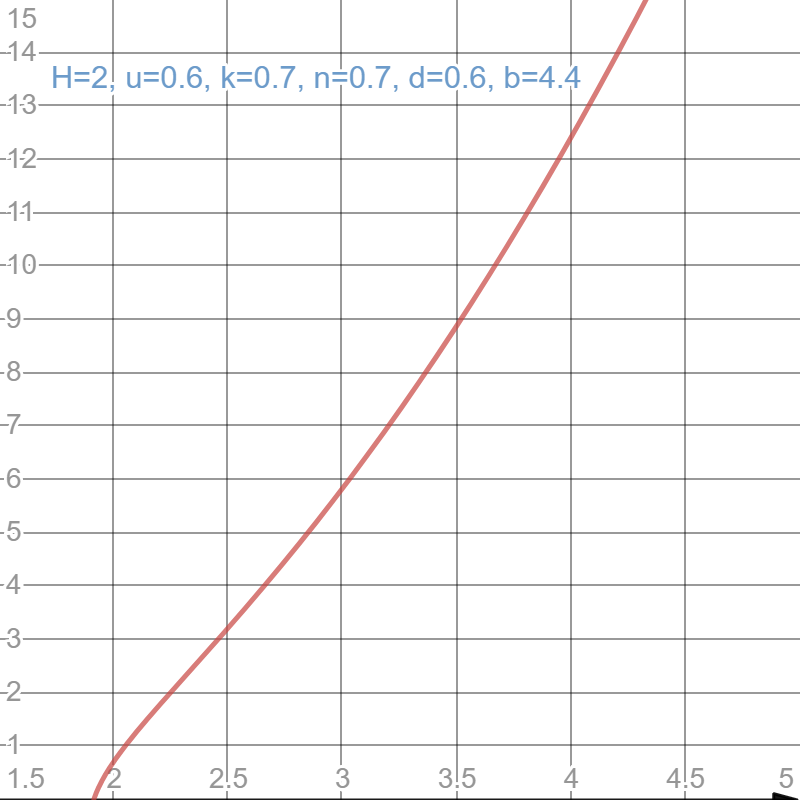
\includegraphics[scale=0.2]{disp-real-base.png}
    \subcaption{Real part of the dispersion relation}
    \label{disp-real-base}
    \end{subfigure}
    \begin{subfigure}{0.5\textwidth}
    \centering
    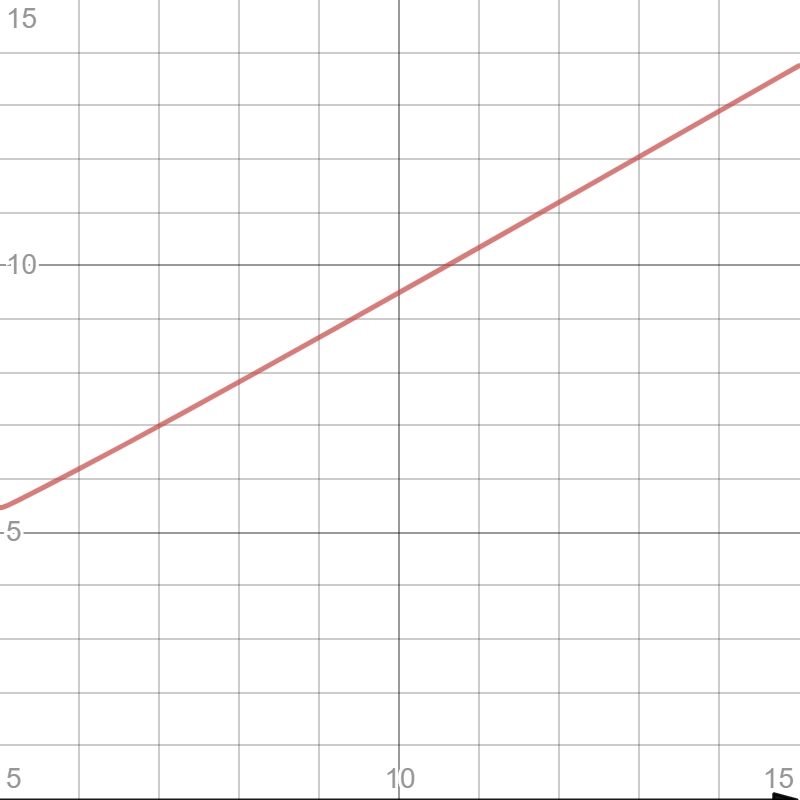
\includegraphics[scale=0.2]{disp_imgwvsk.png}
    \subcaption{Imaginary part of the dispersion relation}
    \label{disp-img-base}
    \end{subfigure}
    \caption{Plots showing the real and imaginary part of the dispersion relation: eq.\eqref{dispersion-final}}
\end{figure}
\begin{figure}[t]
    \begin{subfigure}{0.5\textwidth}
    \centering
    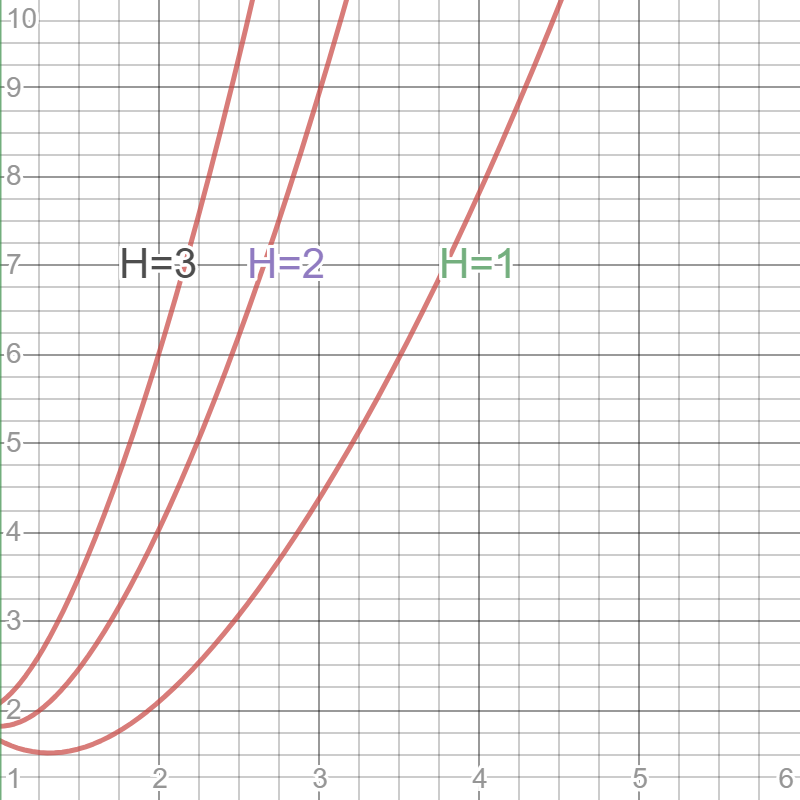
\includegraphics[scale=0.2]{real-disp-Hvar.png}
    \subcaption{Variation with H.}
    %\label{disp-real-H}
    \end{subfigure}
    \begin{subfigure}{0.5\textwidth}
    \centering
    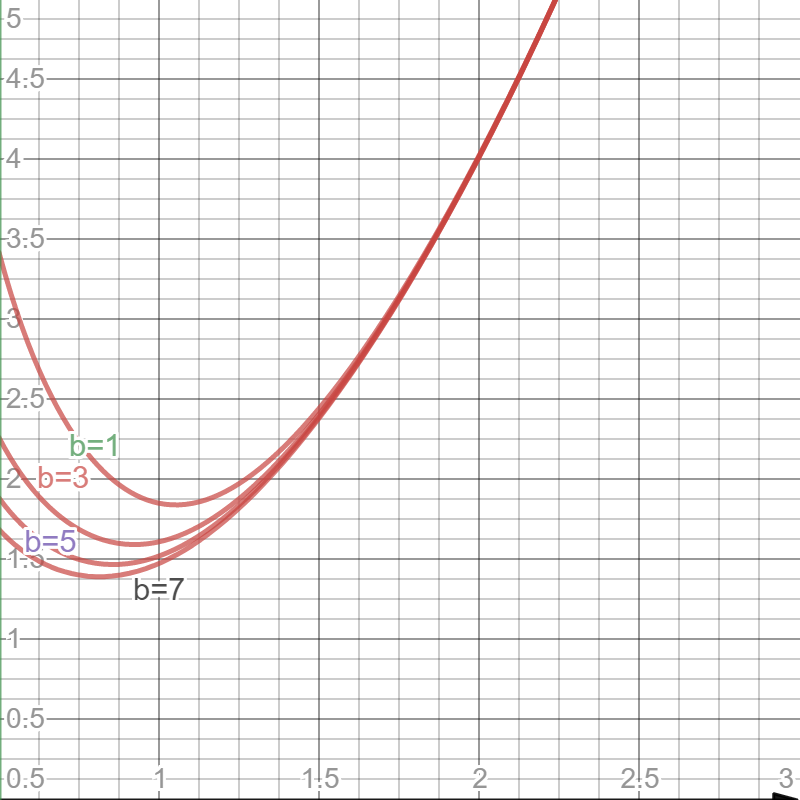
\includegraphics[scale=0.2]{real-disp-b_var.png}
    \subcaption{Variation with $\beta$, identified by b in the graph.}
    %\label{disp-real-beta}
    \end{subfigure}
    \caption{Variation of the dispersion relation with H(Fig. a) and $\beta$(Fig. b).}
    \label{disp-var1}
\end{figure}
\newpage
\section{Shock Waves and the KdV Burgers equation}
\subsection{Reductive perturbation technique}
This technique is used to obtain the shock wave equation in plasma. It involves stretching of the space and time coordinates and then examining the resulting equations in various
orders of smallness(perturbations). The stretching of the coordinates helps in amplification of the already small perturbations. What entails in the following is a case of extreme stretching
such that the space coordinates are stretched by a factor of $\epsilon$ while time coordinate is stretched by a factor of $\epsilon^3$.
\begin{eqnarray}
    \xi &=& \epsilon(x - V_0 t) \label{stretchx}\\
    \tau &=& \epsilon^3 t \label{stretcht}\\
    \eta &=& \epsilon \eta_0 \label{stretcheta}
\end{eqnarray}
The reason for stretching $\eta$ is because, of the way it is normalized. The normalization of $\eta$ is through velocity and frequency. Since the velocity and frequency become stretched, $\eta$ is stretched, quite similar to the process presented in the Appendix section of \cite{jyoti2020}.
Due to the stretching, differentials with respect to time and space change as follows:
\begin{eqnarray}
    \frac{\partial}{\partial t} &=& \epsilon^3 \frac{\partial}{\partial \tau} - \epsilon V_0 \frac{\partial}{\partial \xi} \label{stretch-diff-tau}\\
    \frac{\partial}{\partial x} &=& \epsilon \frac{\partial}{\partial \xi} \label{stretch-diffx}
\end{eqnarray}
Substituting equations \ref{stretch-diffx} and \ref{stretch-diff-tau} in equations \ref{cont-h} - \ref{poisson}, the following are obtained\dots\\
The continuity equations become:
\begin{equation}
    \begin{split}
        (\epsilon^3 \frac{\partial}{\partial \tau} - \epsilon V_0 \frac{\partial}{\partial \xi})(\epsilon {n_j}^{(1)} + \epsilon^2 {n_j}^{(2)} + \dots) +\\
        \epsilon \frac{\partial}{\partial \xi}(1 + \epsilon {n_j}^{(1)} + \epsilon^2 {n_j}^{(2)} + \dots)(u_0 + \epsilon {u_j}^{(1)} + \epsilon^2 {u_j}^{(2)} + \dots)
        =0    
    \end{split}
\end{equation}
\newpage
\begin{figure}[h]
    \begin{subfigure}{0.5\textwidth}
    \centering
    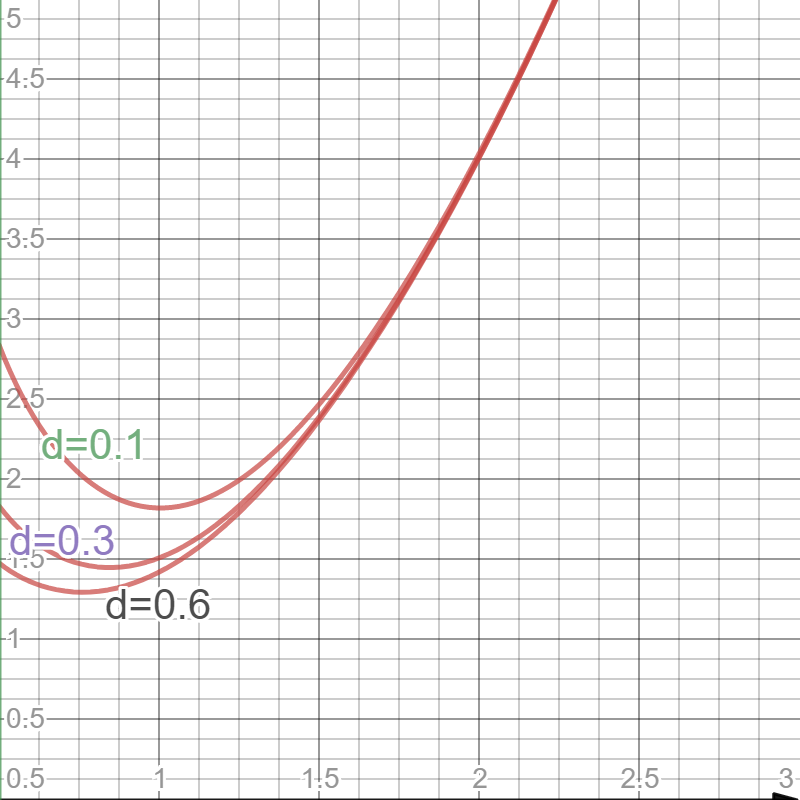
\includegraphics[scale=0.2]{real-disp-d_var.png}
    \subcaption{Variation with $\delta$, identified by b in the graph.}
    \label{disp-real-delta}
    \end{subfigure}
    \begin{subfigure}{0.5\textwidth}
    \centering
    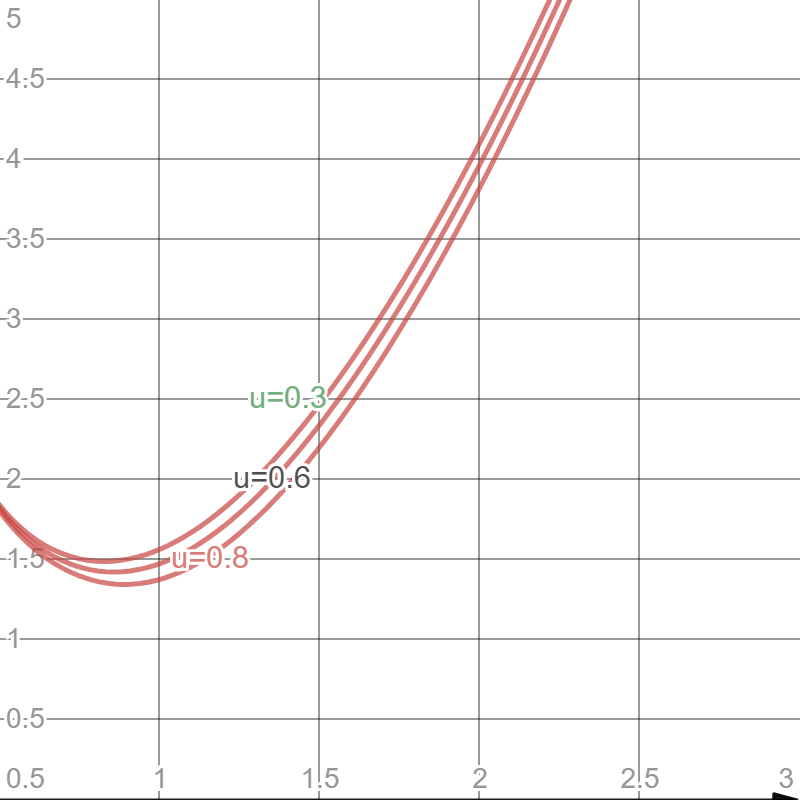
\includegraphics[scale=0.2]{real-disp-u0-var.png}
    \subcaption{Variation with $u_0$, identified by u in the graph.}
    \label{disp-real-u0}
    \end{subfigure}
    \caption{Variation of the dispersion relation with $\delta$(Fig. a) and $u_0$(Fig. b).}
    \label{disp-var2}
\end{figure}
\noindent Taking the terms with varying powers of $\epsilon$
\begin{eqnarray}
    &\epsilon^2:& \quad(u_0-V_0) \frac{\partial {n_j}^{(1)}}{\partial \xi} + \frac{\partial}{\partial \xi}u_j^{(1)} = 0 \label{cont-ep2} \\
    &\epsilon^3:& \quad(u_0 - V_0)\frac{\partial {n_j}^{(2)}}{\partial \xi} + \frac{\partial}{\partial \xi}({n_j}^{(1)}{u_j}^{(1)} + {u_j}^{(2)}) = 0 \label{cont-ep3} \\
    &\epsilon^4:& \quad\frac{\partial {n_j}^{(1)}}{\partial \tau} + (u_0 - V_0)\frac{\partial {n_j}^{(3)}}{\partial \xi} + \frac{\partial}{\partial \xi}({u_j}^{(2)}{n_j}^{(1)} + {u_j}^{(1)}{n_j}^{(2)} + {u_j}^{(3)}) = 0 \label{cont-ep4}
\end{eqnarray}
\newline
The momentum equation for the hot electrons (taking upto first order in Taylor expansion of $\sqrt{n_h}$ or ${n_h}^{-\frac{1}{3}}$) becomes\dots\\
\begin{equation}
    \begin{split}
    0 = \epsilon \frac{\partial}{\partial \xi}(\epsilon \phi^{(1)} + \epsilon^2 \phi^{(2)} + \dots) - 
    \epsilon \beta (1 - \epsilon \frac{{n_h}^{(1)}}{3} - \epsilon^2 \frac{{n_h}^{(2)}}{3} \dots)\frac{\partial}{\partial \xi}(\epsilon {n_h}^{(1)} + \epsilon^2 {n_h}^{(2)} + \dots)\\
    + \epsilon^3 \frac{H^2}{2}\frac{\partial}{\partial \xi}[(1 - \epsilon\frac{{n_h}^{(1)}}{2} - \epsilon^2\frac{{n_h}^{(2)}}{2} \dots)\frac{\partial^2}{\partial \xi^2}(1 + \epsilon\frac{{n_h}^{(1)}}{2} + \epsilon^2\frac{{n_h}^{(2)}}{2} \dots)]    
    \end{split}
\end{equation} 

\noindent Taking the terms with varying powers of $\epsilon$
\begin{eqnarray}
    &\epsilon^2:& \quad 0 = \frac{\partial \phi^{(1)}}{\partial \xi} - \beta\frac{\partial {n_h}^{(1)}}{\partial \xi} \label{mom-h-ep2} \\
    &\epsilon^3:& \quad 0 = \frac{\partial \phi^{(2)}}{\partial \xi} - \beta\frac{\partial {n_h}^{(2)}}{\partial \xi} + \beta\frac{n_h^{(1)}}{3}\frac{\partial n_h^{(1)}}{\partial \xi} \label{mom-h-ep3} \\
    &\epsilon^4:& \quad 0 = \frac{\partial \phi^{(3)}}{\partial \xi} - \beta\frac{\partial n_h^{(3)}}{\partial \xi} + \frac{\beta}{3}\frac{\partial}{\partial \xi}(n_h^{(1)} n_h^{(2)}) + \frac{H^2}{4}\frac{\partial^3 n_h^{(1)}}{\partial \xi^3} \label{mom-h-ep4}
\end{eqnarray} 
\newpage
\noindent The momentum equation for the cold electrons becomes\dots\\
\begin{equation}
    \begin{split}
    (\epsilon^3 \frac{\partial}{\partial \tau} - \epsilon V_0 \frac{\partial}{\partial \xi})(\epsilon {n_c}^{(1)} + \epsilon^2 {n_c}^{(2)} + \dots) +
    \epsilon(u_0 + \epsilon u_c^{(1)} + \dots)\frac{\partial}{\partial \xi}(\epsilon u_c^{(1)} +\dots)\\ = \epsilon\frac{\partial}{\partial \xi}(\epsilon \phi^{(1)} +\dots) +
    \epsilon^3 \frac{H^2}{2}\frac{\partial}{\partial \xi}[(1- \epsilon\frac{n_c^{(1)}}{2} +\dots)\frac{\partial^2}{\partial\xi^2}(1+\epsilon\frac{n_c^{(1)}}{2})] +
    \epsilon^3\eta_0 \frac{\partial^2}{\partial\xi^2}(\epsilon u_c^{(1)} +\dots)
\end{split}
\end{equation}
Taking the terms with varying powers of $\epsilon$
\begin{eqnarray}
    &\epsilon^2:& \quad (u_0 - V_0)\frac{\partial u_c^{(1)}}{\partial\xi} = \frac{\partial\phi^{(1)}}{\partial\xi} \label{mom-c-ep2}\\
    &\epsilon^3:& \quad (u_0 - V_0)\frac{\partial u_c^{(2)}}{\partial\xi} + u_c^{(1)}\frac{\partial u_c^{(1)}}{\partial\xi} = \frac{\partial\phi^{(2)}}{\partial \xi} \label{mom-c-ep3}\\
    &\epsilon^4:& \quad \frac{\partial u_c^{(1)}}{\partial \tau} + (u_0 - V_0)\frac{\partial u_c^{(3)}}{\partial \xi} + \frac{\partial}{\partial \xi}(u_c^{(1)} u_c^{(2)})
    = \frac{\partial \phi^{(3)}}{\partial\xi} + \frac{H^2}{4}\frac{\partial^3 n_c^{(1)}}{\partial\xi^3} + \eta_0\frac{\partial^2 u_c^{(1)}}{\partial\xi^2} \label{mom-c-ep4}
\end{eqnarray}
\newline
\newline
And finally, the Poisson equation becomes\dots
\begin{equation}
    \epsilon^2 \frac{\partial^2}{\partial\xi^2}(\epsilon\phi^{(1)} + \epsilon^2\phi^{(2)}+\dots) = (1+\frac{1}{\delta}-\frac{\delta_1 n_i}{\delta}) + \epsilon (n_c^{(1)} + \frac{n_h^{(1)}}{\delta}) + \epsilon^2 (n_c^{(2)} + \frac{n_h^{(2)}}{\delta}) +\dots    
\end{equation}
Taking terms with varying powers of $\epsilon$
\begin{eqnarray}
     &\epsilon:& \quad n_c^{(1)} + \frac{n_h^{(1)}}{\delta} = 0 \label{poisson-ep1} \\
     &\epsilon^2:& \quad n_c^{(2)} + \frac{n_h^{(2)}}{\delta} = 0 \label{poisson-ep2} \\
     &\epsilon^3:& \quad \frac{\partial^2 \phi^{(1)}}{\partial \xi^2} = n_c^{(3)} + \frac{n_h^{(3)}}{\delta} \label{poisson-ep3} \\
     &\epsilon^4:& \quad \frac{\partial^2 \phi^{(2)}}{\partial\xi^2} = n_c^{(4)} + \frac{n_h^{(4)}}{\delta} \label{poisson-ep4} \\
\end{eqnarray}
Since the second derivative of $\phi^{(2)}$ is related to the fourth order perturbation terms which are already very small,
\begin{equation}
    \frac{\partial\phi^{(2)}}{\partial\xi} = \int (n_c^{(4)} + \frac{n_h^{(4)}}{\delta}) d\xi \notag
\end{equation}
This $\frac{\partial \phi^{(2)}}{\partial \xi}$ term is therefore very small and can be safely neglected in the upcoming equations.\\
%\newpage
\noindent Now, using equations \ref{cont-ep2}, \ref{mom-h-ep2}, \ref{mom-c-ep2}, \ref{poisson-ep1}, all first order perturbations $n_h^{(1)}$, $n_c^{(1)}$, $u_h^{(1)}$ and $u_c^{(1)}$ are obtained in terms of $\phi^{(1)}$.
\begin{eqnarray}
    n_h^{(1)} &=& \frac{\phi^{(1)}}{\beta}\\
    n_c^{(1)} &=& -\frac{\phi^{(1)}}{(V_0 - u_0)^2}\\
    u_h^{(1)} &=& \frac{(V_0 - u_0)}{\beta}\phi^{(1)}\\
    u_c^{(1)} &=& -\frac{1}{(V_0 - u_0)}\phi^{(1)}
\end{eqnarray}
\newline
The terms $u_c^{(2)}$ and $n_c^{(2)}$ may be written in terms of $n_c^{(1)}$ as
\begin{eqnarray}
    u_c^{(2)} &=& \frac{(V_0 - u_0)^2}{2} (n_c^{(1)})^2\\
    n_c^{(2)} &=& \frac{3}{2}(n_c^{(1)})^2
\end{eqnarray}
\newline
By elimination of the third order perturbation terms, and dropping the superscript from $\phi^{(1)}$ the non-linear KdVB equation for the EAWs is obtained.
\begin{equation}\label{final}
    \frac{\partial \phi}{\partial\tau} + p \phi^2 \frac{\partial\phi}{\partial \xi} + r \frac{\partial^3 \phi}{\partial \xi^3} - q \frac{\partial^2 \phi}{\partial \phi^2} = 0
\end{equation}
Where,
\begin{eqnarray}
    p &=& \frac{3}{(V_0 - u_0)^4} + \frac{\delta^2}{12} \frac{1}{(V_0 - u_0)^3} + \frac{1}{2(V_0 - u_0)^3} \notag \\
    q &=& \frac{\eta}{2} \notag \\
    r &=& \frac{\delta H^2}{8 \beta} + \frac{(V_0 - u_0)^3}{2} + \frac{H^2}{8} \frac{1}{(V_0 - u_0)} \notag
\end{eqnarray}

\subsection{Solution to the modified KdV-Burgers equation}
Travelling wave solutions are desired from equation (\ref{final}), since these are physically relevant to the investigation.
There are multiple possible ways to obtain such solutions, such as the tanh-sech method[ref something], homogeneous balance method\cite{fan-zhang}, extended tanh method\cite{wazwaz2008}.\\
\indent While the tanh method introduced by Malfiet\cite{malfliet-hereman} is a reliable way to tret nonlinear wave equations, the extended tanh method is a more direct method.
Not going through the entire process of derivation of the solutions, the results obtained by Bekir\cite{bekir} are directly stated for the modified KdV-Burgers equation.
There are three possible solutions to the equation.
\begin{eqnarray}
    \phi_1 &=& \pm \sqrt{\frac{6r}{p}}[ 1 + coth(x - 8rt)] \notag \\
    \phi_2 &=& \pm \sqrt{\frac{6r}{p}}[ 1 + tanh(x - 8rt)] \notag \\
    \phi_3 &=& \pm 3\sqrt{\frac{6r}{p}}[ 2 + tanh(x - 32rt) + coth(x - 32rt)] \notag
\end{eqnarray}

\begin{figure}[t]
\begin{subfigure}{0.5\textwidth}
\centering
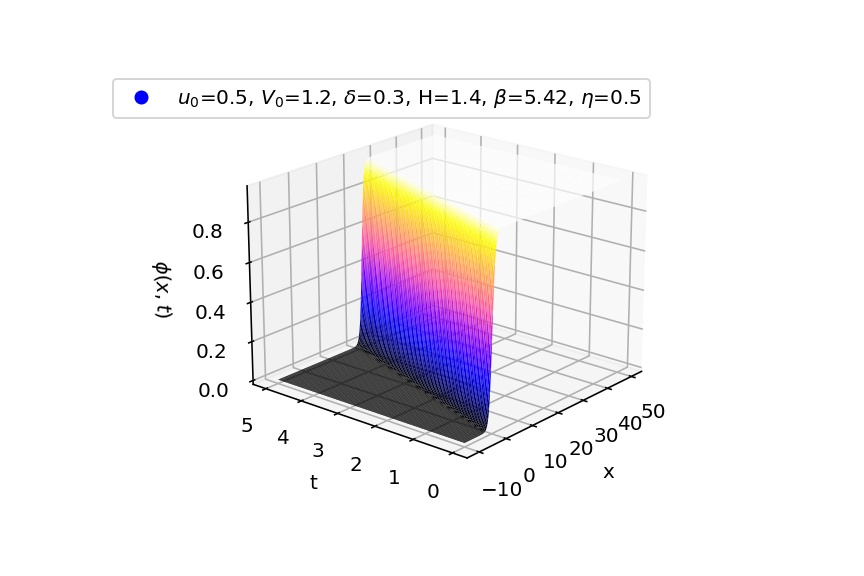
\includegraphics[scale=0.7]{tanh_t0--5.jpg}
\subcaption{Positions of wave in time interval 0 to 5}
\label{fig1}
\end{subfigure}
\begin{subfigure}{0.5\textwidth}
\centering
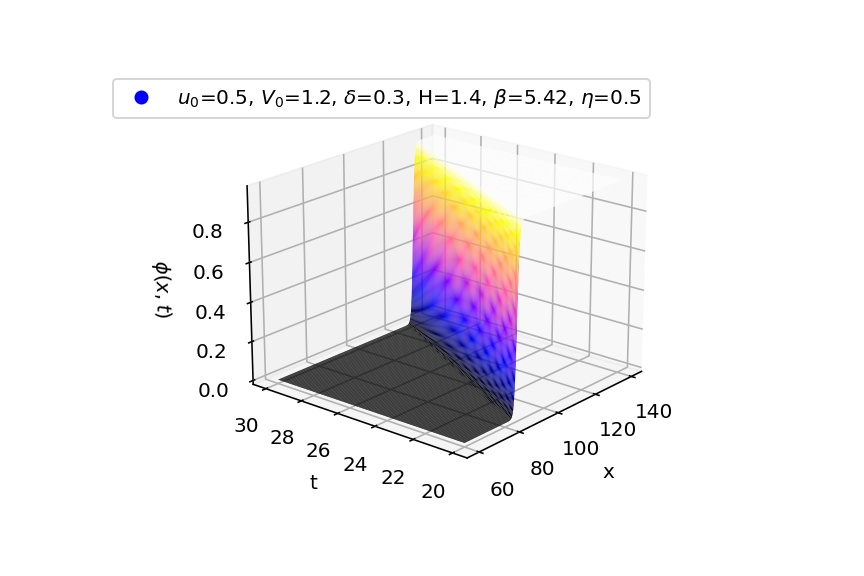
\includegraphics[scale=0.7]{tanh_t20--30.jpg}
\subcaption{Positions of wave in time interval 20 to 30}
\label{fig2}
\end{subfigure}
\caption{This is the plot of $\phi_2$ with respect to space and time, showing the propagation of the wave with time. The parameters of the plasma are given in the graphs}
\label{tanh}
\end{figure}
From these three possible solutions, $\phi_2$ is used from now on. Plots of positive values of $\phi_2$ are shown at the top in Fig. \ref{tanh}. The two graphs show how the wave is travelling through space and time. The KdV-Burgers equation obtained in eq.\eqref{final} is a special kind of equation since the solution to this in not like the solitons obtained from a normal KdV equation. Here the wave progress unaltered with a fixed velocity. So the location of the wave can simply be shown on the x-t plane, as a straight line whose slope gives the speed of the travelling wave. Judging by this nature, it is imperative that the plasma parameters mainly affect the amplitude of the wave, when a single soliton is involved. Same occurs for the negative solution of $\phi$, which is why it is ignored.
\begin{figure}[h]
    \begin{subfigure}{0.5\textwidth}
    \centering
    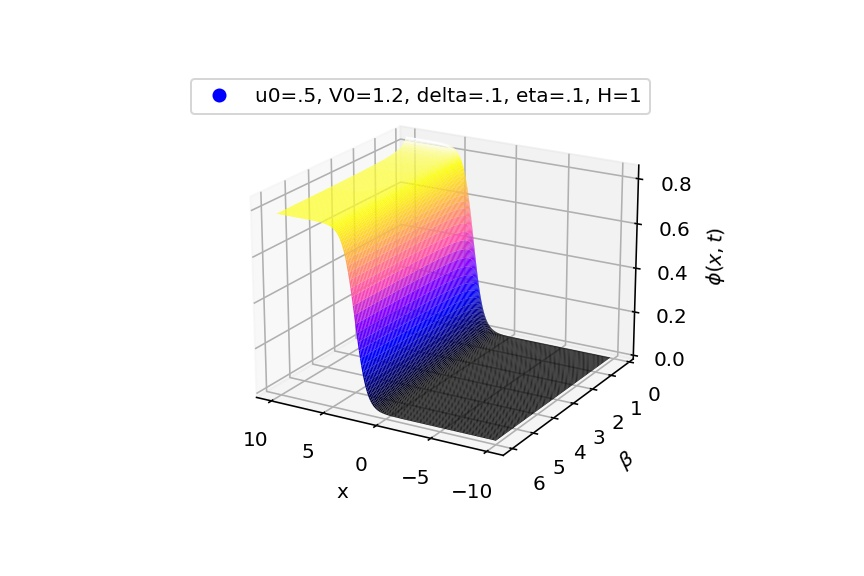
\includegraphics[scale=0.5]{tanh_phivsBeta.jpg}
    \subcaption{Variation of the wave with $\beta$.}
    \label{plot-beta}
    \end{subfigure}
    \begin{subfigure}{0.5\textwidth}
    \centering
    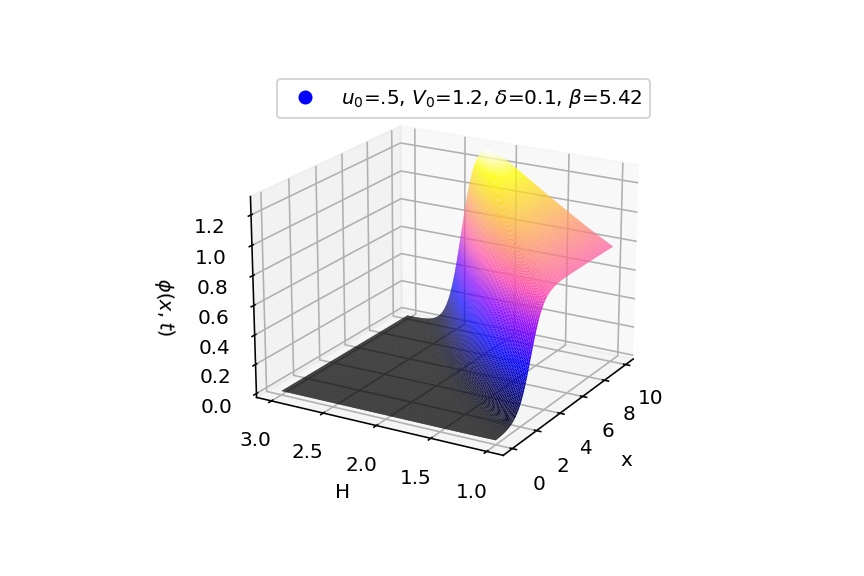
\includegraphics[scale=0.5]{tanh_phivsH.jpg}
    \subcaption{Variation of the wave with H.}
    \label{plot-H}
    \end{subfigure}
    %\caption{Caption}
    %\label{plot-phiVSvars1}
%\end{figure}
%\begin{figure}[t]
    \begin{subfigure}{0.5\textwidth}
    \centering
    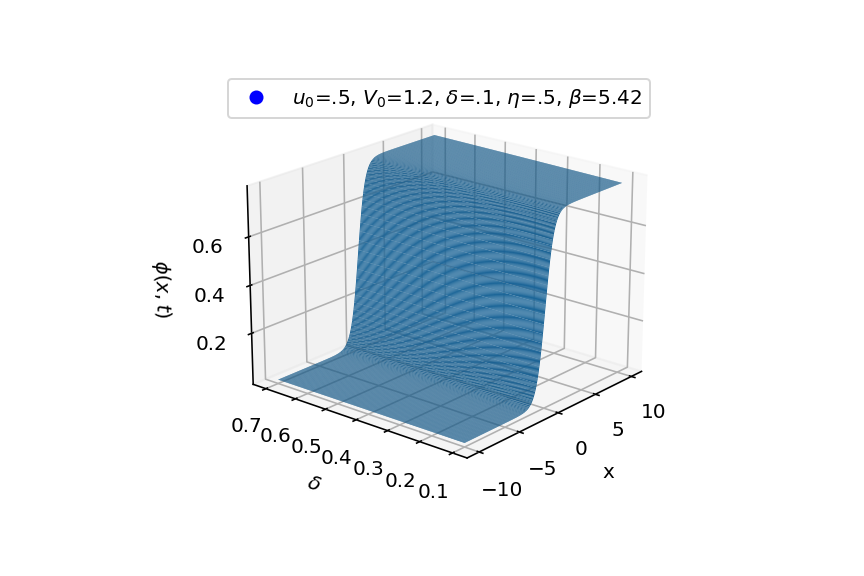
\includegraphics[scale=0.5]{tanh_phivsDelta.png}
    \subcaption{Variation of wave with $\delta$.}
    \label{plot-delta}
    \end{subfigure}
    \begin{subfigure}{0.5\textwidth}
    \centering
    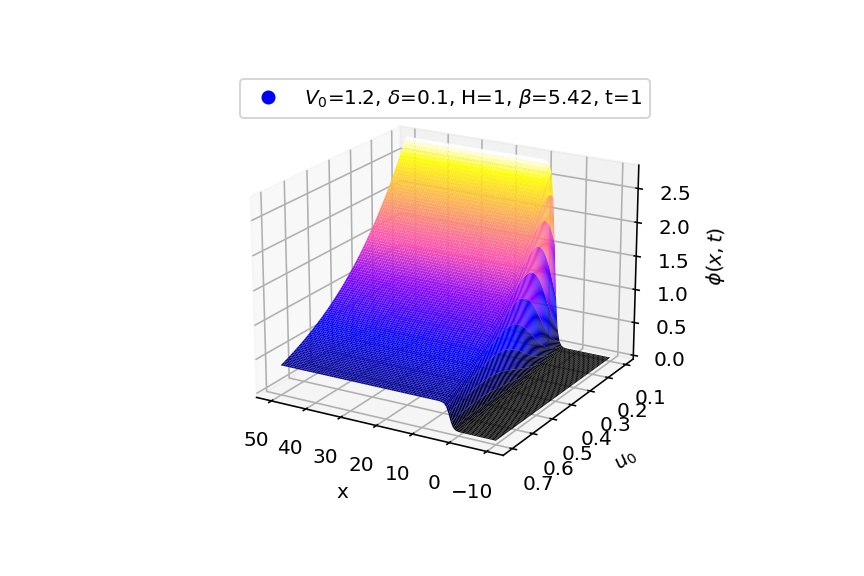
\includegraphics[scale=0.5]{tanh_phivsU0.jpg}
    \subcaption{Variation of wave with $u_0$.}
    \label{plot-u0}
    \end{subfigure}
    \caption{Variation of the amplitude of the travelling wave with change of plasma parameters.}
    \label{plot-phiVSvars1}
\end{figure}
Following plots describe something..
\begin{figure}[t]
    \centering
    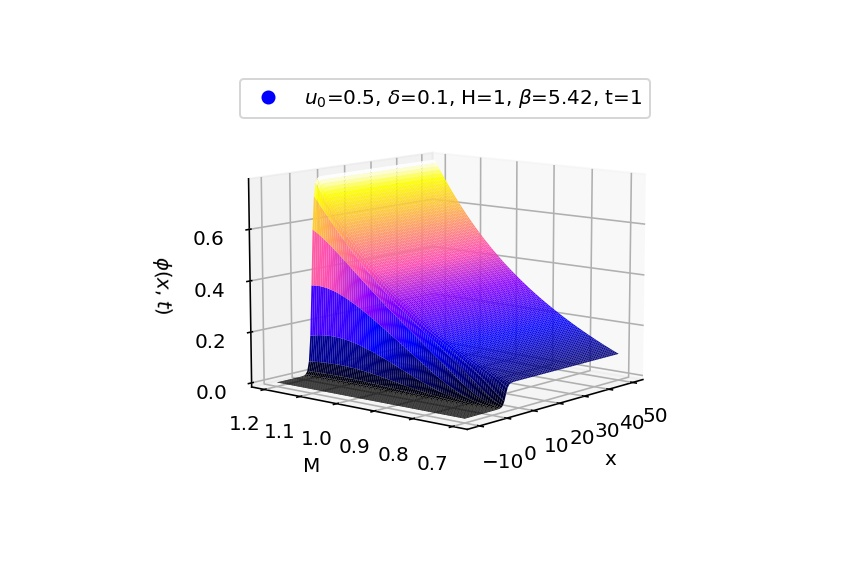
\includegraphics[scale=1]{tanh_phivsV_0.jpg}
    \caption{vs Mach Number}
    \label{plot-delta}
\end{figure}
\newpage
\subsection{Numerical simulation of the modified KdV-Burgers equation}
Given how powerful computers have become in the last couple of years, it would be a shame to not carry out a numerical simulation of the nonlinear equation (\ref{final}). There are a plethora of options available for numerically solving
differential equations, the simplest being Euler's method, using forward/backward/central difference methods. A more sophisticated approach is through the use of RK4 algorithm. The first computational solution to this equation was given by Zabusky and Krushkal[reference here] in 1965, using a periodic boundary condition which was again justified in another paper by Zabusky\cite{Zabusky1971}. However, there are also other convergence criteria involved in its solution,
which implies that just applying a difference equation won't work, specially when third order derivatives are involved. The approach used here is a Fourier transform - split step method\cite{muslu2003}, which is well applicable for nonlinear
equations like the KdV or mKdV. The algorithm goes as follows\dots
\newline
\newline
Equation (\ref{final}) can be written in a compact form as:
\begin{equation}\label{final-compact}
    \partial_\tau \phi + p \phi^2 \partial_\xi \phi + r \partial_{\xi\xi\xi} \phi - q\partial_{\xi\xi} \phi = 0
\end{equation}
Taking a Fourier transform
\begin{equation}
    d_\tau \tilde{\phi} + \frac{p}{3} (ik) \widetilde{\phi^3} + r {(ik)}^3 \tilde{\phi} - q {(ik)}^2 \tilde{\phi} = 0 \label{Fouriated}
\end{equation}
Where $\tilde{\phi}$ is the Fourier transform of $\phi$ while $\widetilde{\phi^3}$ is the Fourier transform of $\phi^3$.\\
Now Simplifying\dots
\begin{equation}
    d_\tau \tilde{\phi} = -\frac{p}{3}(ik)\widetilde{\phi^3} + i r k^3 \tilde{\phi} + q k^2\tilde{\phi} \label{mini-fouriated}
\end{equation}
The linear and nonlinear part of this equation is treated separately:
\begin{eqnarray}
    d_\tau \tilde{\phi}(k, t) &=& (irk^3 - qk^2)\tilde{\phi}(k,t) \label{fouriated-linear}\\
    \implies \tilde{\phi}(k,t) &=& \tilde{\phi}(k)e^{(irk^3 - qk^2)t} \label{fouriated-int}\\
    d_\tau \tilde{\phi}(k, t) &=& -\frac{p}{3}(ik) \widetilde{\phi^3}(k,t) \label{fouriated-nonlin}
\end{eqnarray}
Equation (\ref{fouriated-linear}) handles the linear part of eq\ref{mini-fouriated}, while \ref{fouriated-nonlin} handles the nonlinear part.
Now, from equation (\ref{fouriated-int}), let
\begin{equation}
    \tilde{\phi_1}(k, t+\varDelta t) = \tilde{\phi}(k,t) e^{(irk^3 - qk^2)\varDelta t} \label{fouriated-semifinal}
\end{equation}
Using a similar expansion as the principle of differentiation on equation (\ref{fouriated-nonlin})\dots
\begin{equation}
    \tilde{\phi}(k, t + \varDelta t) = \tilde{\phi_1}(k, t + \varDelta t) 
    - \frac{ipk}{3} \Biggl[ F {\Biggl(F^{-1}\Bigl( \tilde{\phi_1}(k, t + \varDelta t)\Bigr) \Biggr)}^3\Biggr] \label{fouriated-final}
\end{equation}
Here, $F$ denotes the Fourier transform operator, while $F^{-1}$ denotes the inverse-Fourier transform operator. Application of equations (\ref{fouriated-semifinal}) and (\ref{fouriated-final})
iteratively within a given time range and taking its real value, the value of $\phi$ is obtained\footnote{A matlab script is provided at ...}.
\newpage
\bibliographystyle{plain}
\bibliography{ref}
\end{document}